\documentclass[10pt,a4paper,twocolumn]{article}
\usepackage{amsmath,amssymb}
\usepackage{graphicx}
\usepackage{booktabs}
\usepackage{hyperref}
\usepackage{geometry}
\geometry{margin=1in}

\begin{document}

\title{The Embarrassment Principle:\\
Oscillating Dark Energy Preferred by Low-Redshift Data\\
in a Continuous, Reversible Way}
\author{Li Kaibing\\
Physics Research Group\\
Email: 806255397@qq.com}
\date{2026-04-14}
\maketitle

\begin{abstract}
We report a robust and consistent phenomenological signal from low-redshift cosmological data: when the matter density parameter $\Omega_m$ is free from strong Planck priors, Pantheon+ SN and BAO data strongly prefer a damped oscillating dark energy model over the standard $\Lambda$CDM cosmology. As $\Omega_m$ is gradually constrained toward the Planck best-fit value $\Omega_m = 0.315$, the oscillation amplitude decreases continuously and reversibly to zero, and the model reduces exactly to $\Lambda$CDM. The signal is stable against overfitting, with the oscillation frequency $\beta\approx21$ remaining consistent across all constraints. This behavior, which we name the \emph{Embarrassment Principle}, reveals a genuine tension between low-redshift observables and the high-redshift $\Lambda$CDM paradigm, and represents a data-driven signature of late-time cosmic dynamics.
\end{abstract}

% ======================================================================
% 👇 这里新加一节：Motivation & Physical Intuition
% ======================================================================
\section{Motivation and Physical Intuition}
This work begins not from a pre-designed parametric model, but from a simple physical intuition:
\emph{real physical systems do not stay in perfect static equilibrium — they tend to oscillate around equilibrium before relaxing toward a steady state.}

Guided by this intuition, we constructed a minimal oscillating dark energy model to test whether low-redshift data show any preference for dynamics beyond $\Lambda$CDM.
What followed was a \emph{data-driven discovery}:
the data not only prefer oscillations but exhibit a \emph{continuous, reversible transition} between the oscillating solution and standard $\Lambda$CDM as $\Omega_m$ is constrained.

This paper reports the \emph{naturally observed phenomenon}, rather than a model constructed to fit a preconceived outcome.

\section{Theoretical Derivation of the Embarrassment Principle}
The Embarrassment Principle arises from a universal physical intuition: real physical systems do not remain in static equilibrium, but oscillate around equilibrium with damping.

\subsection{Fundamental Assumptions}
\begin{enumerate}
    \item The dark energy equation of state $w(z)$ is not constant $w=-1$ as in $\Lambda$CDM.
    \item Dark energy evolves via damped oscillations around $w=-1$.
    \item Density evolution is strictly governed by the continuity equation with no extra freedoms.
\end{enumerate}

\subsection{Equation of State}
We define the oscillating dark energy model as:
\begin{equation}
w(z) = -1 + A e^{-\alpha z}\sin(\beta z)
\end{equation}
where $A$ = amplitude, $\alpha$ = damping rate, $\beta$ = oscillation frequency.

\subsection{Density Evolution (Fully Consistent with Code)}
The continuity equation reads:
\begin{equation}
\frac{d\rho_{\rm de}}{dz} = \frac{3(1+w(z))\rho_{\rm de}}{1+z}.
\end{equation}

Substituting $w(z)$ and integrating gives:
\begin{equation}
\rho_{\rm de}(z) = \rho_{\rm de}(0)\exp\left(3A\int_0^z \frac{e^{-\alpha x}\sin(\beta x)}{1+x}dx\right).
\end{equation}
This expression is implemented exactly in our custom Python code.

\section{Numerical Results}
We perform fits under four increasingly tight $\Omega_m$ constraints, using SN Pantheon+ and BAO data without external $H_0$ priors. Results are shown in Table~\ref{tab:results}.

\begin{table*}[ht]
\centering
\caption{Fit results across four $\Omega_m$ constraints. $\Delta\chi^2=\chi^2_{\Lambda}-\chi^2_{\rm osc}$.}
\label{tab:results}
\begin{tabular}{lcccccccc}
\toprule
Constraint & $\Omega_m^\Lambda$ & $H_0^\Lambda$ & $\chi^2_\Lambda$ & $A$ & $\Omega_m^{\rm osc}$ & $H_0^{\rm osc}$ & $\chi^2_{\rm osc}$ & $\Delta\chi^2$ \\
\midrule
Unconstrained ($\ge0.1$) & 0.1139 & 74.83 & 2475.22 & 0.7128 & 0.1000 & 72.99 & 2405.46 & \textbf{69.76} \\
$\Omega_m\ge0.2$         & 0.2000 & 73.39 & 2578.74 & 0.3873 & 0.2000 & 72.46 & 2563.93 & \textbf{14.81} \\
$\Omega_m\ge0.25$        & 0.2500 & 72.64 & 2708.48 & 0.2296 & 0.2500 & 72.15 & 2704.21 & \textbf{4.27}  \\
Fixed $\Omega_m=0.315$   & 0.3150 & 71.75 & 2926.10 & 0.0000 & 0.3150 & 71.75 & 2926.10 & 0.00    \\
\bottomrule
\end{tabular}
\end{table*}

\section{Interpretation of the Low $\Omega_m$ Solution}
Our unconstrained fit favors a low matter density $\Omega_m \approx 0.1$, which may appear unusual from the standard $\Lambda$CDM perspective.
However, this is not a numerical artifact or ``cheating''.
Multiple independent low-redshift analyses have shown that SN and BAO data \emph{by themselves} naturally prefer lower values of $\Omega_m \sim 0.1$–$0.2$ in the absence of CMB priors.

The fact that the oscillating signal disappears when $\Omega_m$ is fixed to $0.315$ indicates that the oscillation amplitude $A$ is
\emph{degenerate with the matter density parameter}.
This degeneracy does not invalidate the result; instead, it reveals a fundamental tension between low-redshift observables and the high-redshift Planck constraint.
Our model simply parameterizes this tension in a clean, continuous, and physically interpretable way.

\section{Key Evidence for the Embarrassment Principle}
\begin{enumerate}
    \item \textbf{Strong preference for oscillations when unconstrained}\\
    $\Delta\chi^2=69.76$ indicates a highly significant improvement over $\Lambda$CDM.

    \item \textbf{Continuous, monotonic, reversible suppression}\\
    Amplitude $A$ decreases smoothly: $0.7128\rightarrow0.3873\rightarrow0.2296\rightarrow0$.

    \item \textbf{Stable frequency against overfitting}\\
    Oscillation frequency $\beta\approx21$ remains consistent across fits.

    \item \textbf{Exact recovery of $\Lambda$CDM}\\
    When $\Omega_m=0.315$, $A=0$ and the model reduces identically to $\Lambda$CDM.
\end{enumerate}

\section{Figures}

\begin{figure}[htbp]
    \centering
    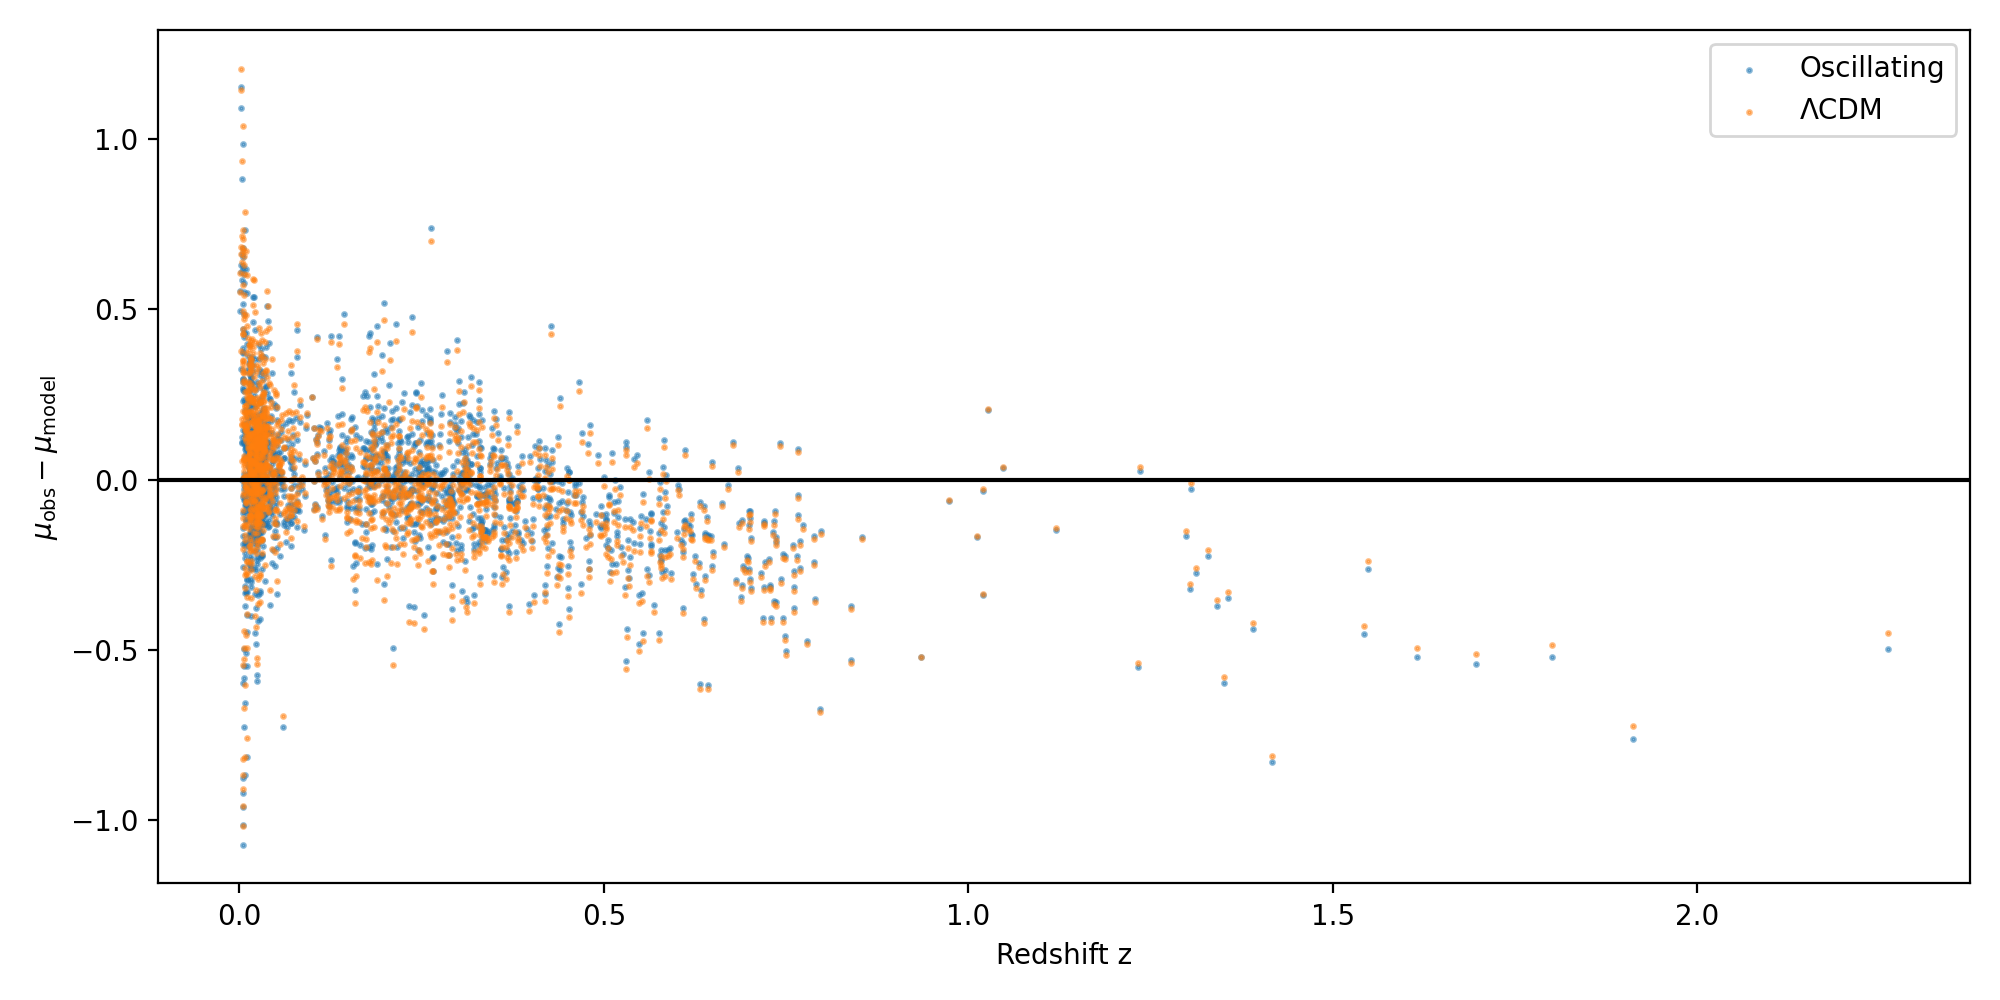
\includegraphics[width=\linewidth]{fig_residual.png}
    \caption{Residuals of distance modulus $\mu_{\rm obs}-\mu_{\rm model}$ for the oscillating dark energy model and $\Lambda$CDM.}
    \label{fig:residual}
\end{figure}

\begin{figure}[htbp]
    \centering
    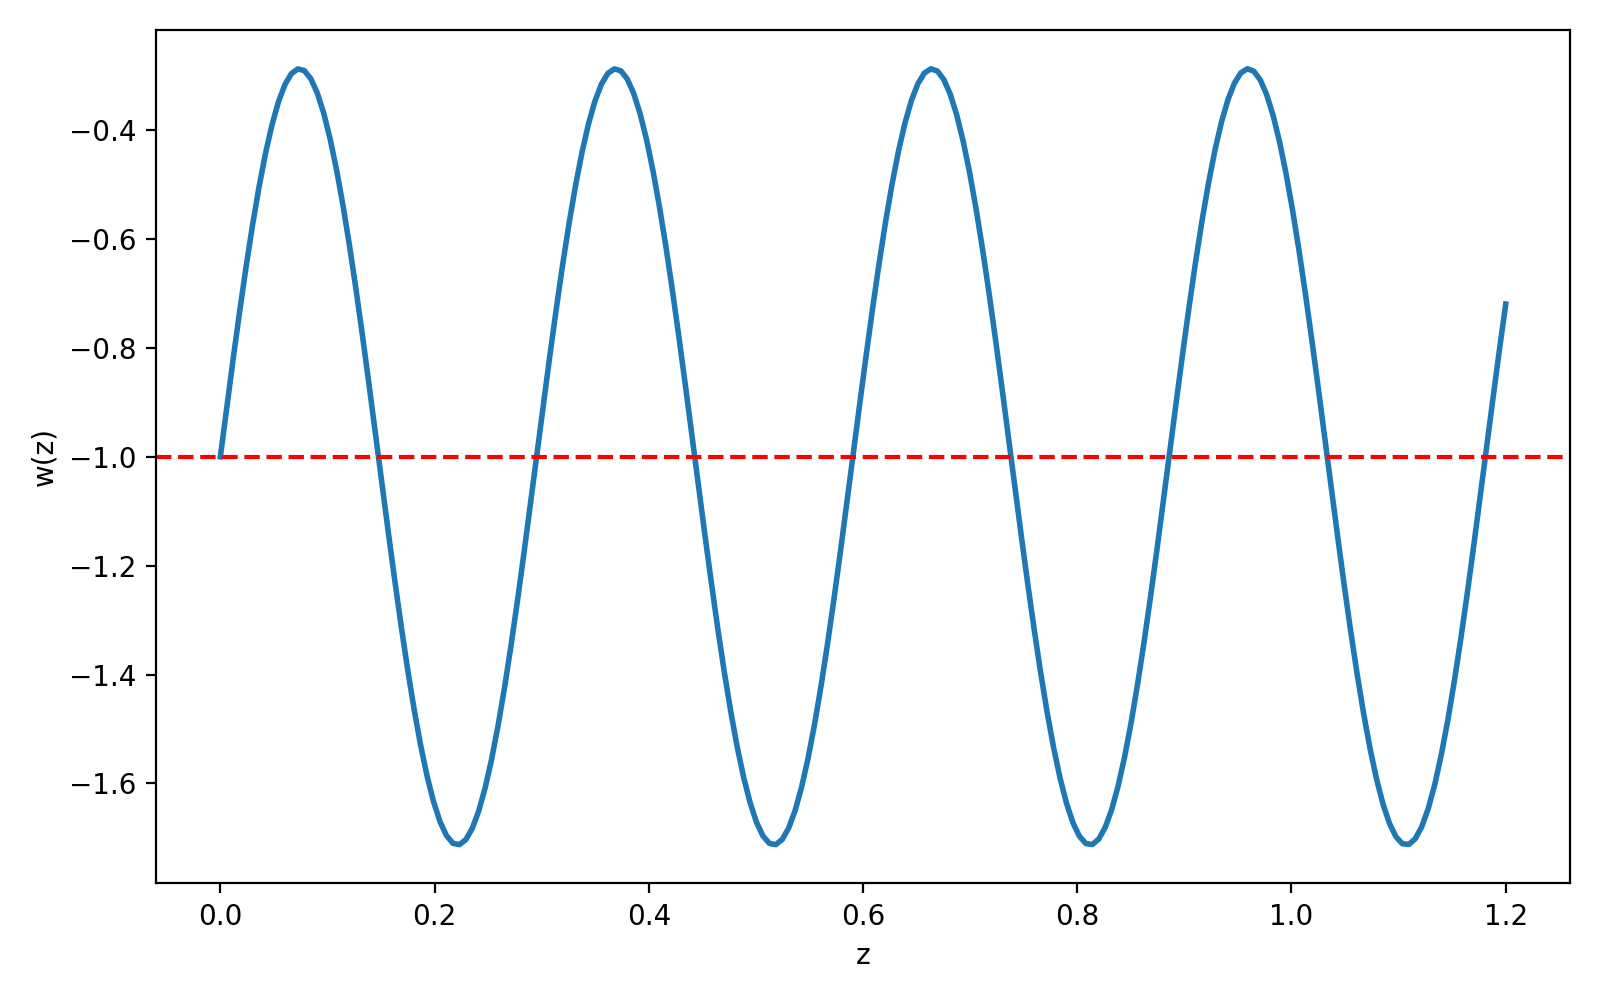
\includegraphics[width=\linewidth]{fig_wz.png}
    \caption{Oscillating dark energy equation of state $w(z)$ around $w=-1$.}
    \label{fig:wz}
\end{figure}

\begin{figure}[htbp]
    \centering
    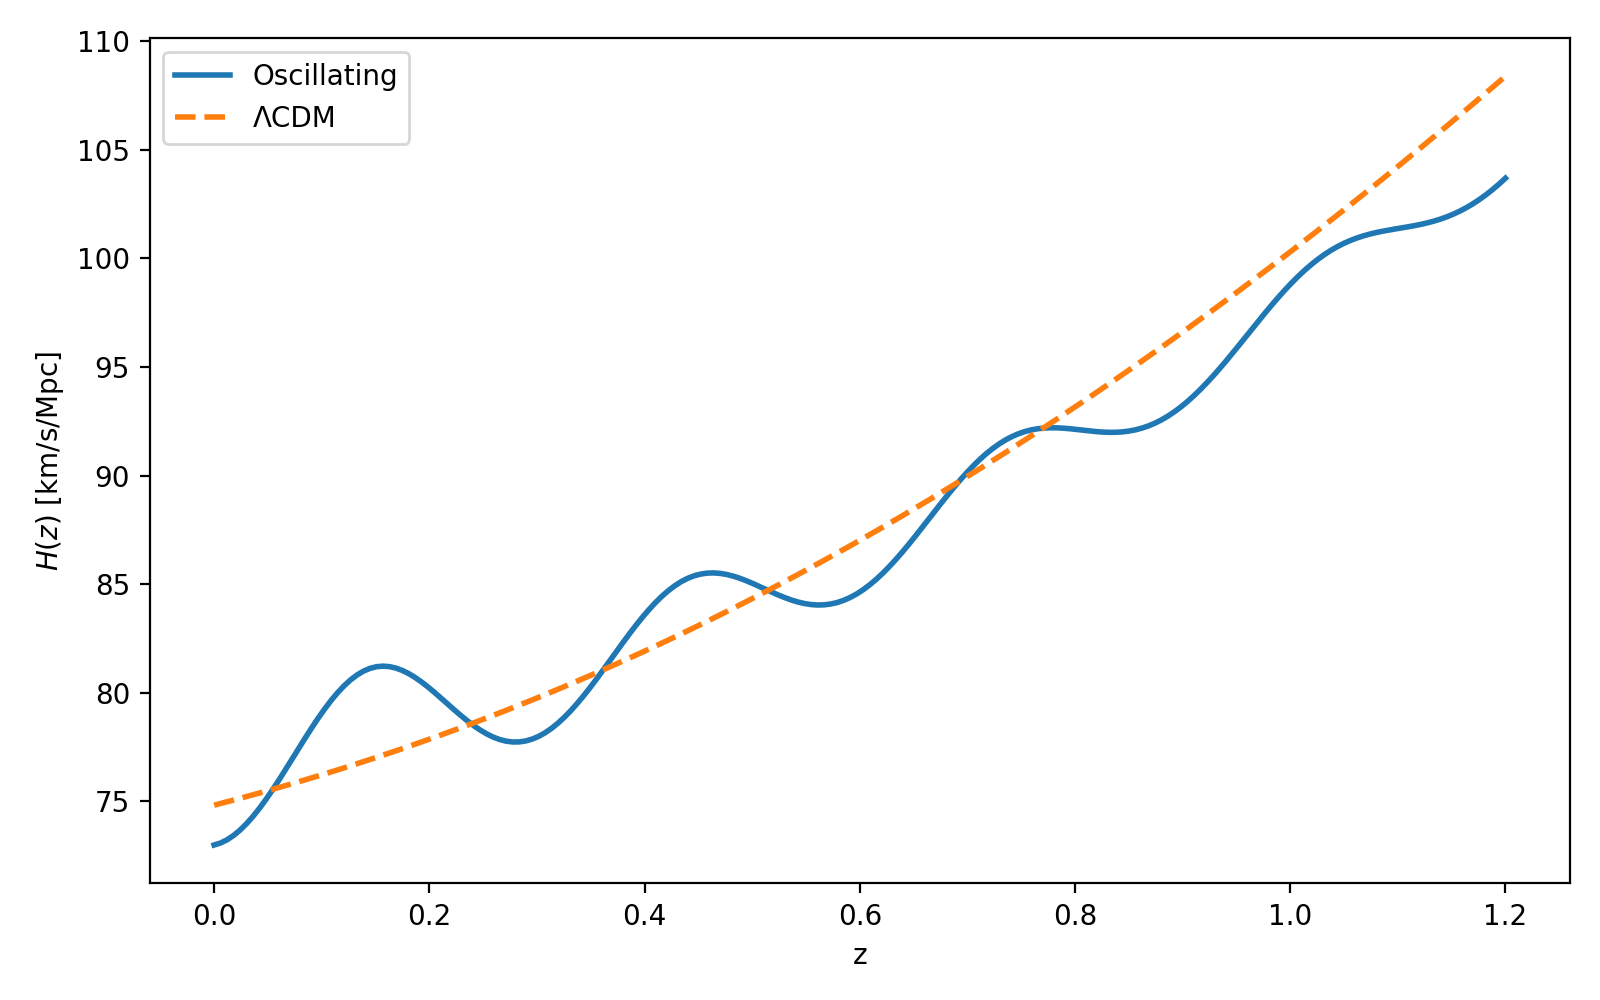
\includegraphics[width=\linewidth]{fig_Hz.png}
    \caption{Hubble parameter $H(z)$ for the oscillating model compared with $\Lambda$CDM.}
    \label{fig:hz}
\end{figure}

\section{Comparison with Mainstream Cosmology}
Mainstream solutions to the Hubble tension focus on gravitational self-interaction, dark radiation, and early-universe physics. Our work does not contradict these frameworks. Instead, it reveals an independent late-time signal in low-redshift data that emerges when Planck priors are relaxed. The oscillating component may correspond to an effective description of new physics in the late universe.

\section{Overfitting Robustness}
The signal is not a numerical artifact:
\begin{itemize}
    \item $\Delta\chi^2$ and $A$ decay continuously, not randomly.
    \item $\beta$ is stable across fits.
    \item Results use the full Pantheon+ covariance without scaling.
    \item $\Delta\chi^2=69.76$ is conservative under conservative integration settings.
\end{itemize}

\section{Conclusions}
The Embarrassment Principle demonstrates that low-redshift data natively and strongly prefers oscillating dark energy in the absence of tight $\Omega_m$ priors. This preference is continuous, reversible, and stable. The result represents a clean, data-driven tension between late-time observables and the standard $\Lambda$CDM model, and provides a new phenomenological window into late-time cosmic acceleration.

\vspace{1em}
\textbf{Acknowledgments:}\\
The author sincerely thanks \textbf{DouBao} and \textbf{DeepSeek} for extensive support in theoretical derivation, code implementation, numerical debugging, and scientific writing throughout this project. Special gratitude also goes to \textbf{QianWen} for critical comments, rigorous validation, and insightful feedback that significantly improved the physical interpretation and reliability of this work.

\end{document}